\section{First problem}
\label{sec:p1}

A single tile is decorated with a machine which is programmed using function 
$f:[0,1] \mapsto [0,1]$. The problem \cite{exam1} claims the final graph $\Lambda$ is
a closed curve, we want to prove it first (just for fun, since this is not required).

Before doing so, we want to find the expressions of $f_1$, $f_2$ and $f_3$: respectively
the symmetrical copies of $f$ on the vertical axis, the horizontal axis and the center 
of coordinates: $O \equiv (0,0)$.
%
% Figure
%-----------------------------------------------------------
%
% One column figure
%-----------------------------------------------------------
   \begin{figure}
   \centering
\tikzstyle{smallfig}=[scale=0.25]
   %
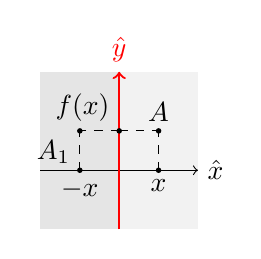
\begin{tikzpicture}[style=smallfig]
\fill [lightgray!20] (0, -3) rectangle (4, 5);
\fill [lightgray!40] (-4, -3) rectangle (0, 5);

\draw[thin,->] (-4,0) -- (4,0) node[right] {$\hat{x}$};
\draw[thick,->,red] (0,-3) -- (0,5) node[above] {$\hat{y}$};

\fill (2,2) circle (4pt) node[above] {$A$};
\draw[dashed,thin,-] (0,2.0) -- (2,2.0);
\fill (0,2) circle (4pt) node[above left] {$f(x)$};
\draw[dashed,thin,-] (2,0) node[below] {$x$} -- (2,2);
\fill (2,0) circle (4pt);
\fill (-2,2) circle (4pt) node[below left] {$A_1$};
\draw[dashed,thin,-] (0,2.0) -- (-2,2.0);
\draw[dashed,thin,-] (-2,0) node[below] {$-x$} -- (-2,2);
\fill (-2,0) circle (4pt);
\end{tikzpicture}
\quad
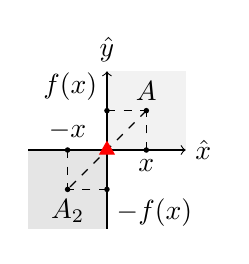
\begin{tikzpicture}[style=smallfig]
\fill [lightgray!20] (0, 0) rectangle (4, 4);
\fill [lightgray!40] (-4, -4) rectangle (0, 0);

\draw[thin,->] (-4,0) -- (4,0) node[right] {$\hat{x}$};
\draw[thin,->] (0,-4) -- (0,4) node[above] {$\hat{y}$};

\fill (2,2) circle (4pt) node[above] {$A$};
\draw[dashed,thin,-] (0,2.0) -- (2,2.0);
\fill (0,2) circle (4pt) node[above left] {$f(x)$};
\draw[dashed,thin,-] (2,0) node[below] {$x$} -- (2,2);
\fill (2,0) circle (4pt);
\fill (-2,-2) circle (4pt) node[below] {$A_2$};
\draw[dashed,thin,-] (0,-2) node[below right] {$-f(x)$} -- (-2,-2);
\draw[dashed,thin,-] (-2,0) node[above] {$-x$} -- (-2,-2);
\fill (0,-2) circle (4pt);
\draw[dashed,thin,-] (2,2) -- (-2,-2);
\fill (-2,0) circle (4pt);

\node[mark size=3pt,color=red] at (0,0) {\pgfuseplotmark{triangle*}};
\end{tikzpicture}
\quad
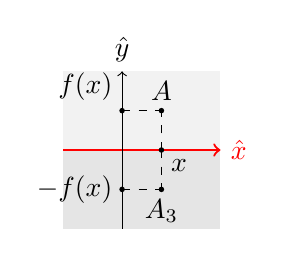
\begin{tikzpicture}[style=smallfig]
\fill [lightgray!20] (-3, 0) rectangle (5, 4);
\fill [lightgray!40] (-3, -4) rectangle (5, 0);

\draw[thick,->,red] (-3,0) -- (5,0) node[right] {$\hat{x}$};
\draw[thin,->] (0,-4) -- (0,4) node[above] {$\hat{y}$};

\fill (2,2) circle (4pt) node[above] {$A$};
\draw[dashed,thin,-] (0,2.0) -- (2,2.0);
\fill (0,2) circle (4pt) node[above left] {$f(x)$};
\draw[dashed,thin,-] (2,0) node[below right] {$x$} -- (2,2);
\fill (2,0) circle (4pt);
\fill (2,-2) circle (4pt) node[below] {$A_3$};
\draw[dashed,thin,-] (2,0) -- (2,-2);
\draw[dashed,thin,-] (0,-2) node[left] {$-f(x)$} -- (2,-2);
\fill (0,-2) circle (4pt);
\end{tikzpicture}
   %
   \caption{The three symmetrical copies of $f$. From left to
    right: vertical, center and horizontal symmetries.}
   \label{fig:symms}
   \end{figure}
%-----------------------------------------------------------
%
%-----------------------------------------------------------
%
Figure \ref{fig:symms} shows this simple calculation.

\begin{proposition}[$\Lambda$ is a closed curve]
\label{lem:lclosed}
Let $f:[0,a] \mapsto [0,a]$, with $a > 0$, be a continuous function also satisfying:
\begin{equation}
\label{eq:fconds}
f(0)=a \wedge f(a)=0 \wedge 0 < f(x) < a, \forall x \in [0,a]
\end{equation}
Then graph $\Lambda$, obtained by adjoining together $\Gamma$ ($f$'s graph) and
its vertically, horizontally and centered symmetries, is a closed curve.
\begin{proof}
Since $\Lambda$ is constructed using $\Gamma$, given that symmentry is an 
isometric\footnote{An isometry is a transformation that does not change distances and
preserves shapes.} 
transformation and that $f$ is continuous (therefore $\Gamma$ is a continuous curve
with no interruptions), then the single thing to prove is that the points were
the copies of $\Gamma$ connect with each other are continuous. We have 4
copies of $\Gamma$:
\begin{equation*}
\begin{array}{c|c|c|c}
\text{\# Quarter} & \text{\# Ranges} & \text{Graph} & \text{\# Function} \\
\hline
\text{I (NE)} & [0,a] \times [0,a] & \Gamma & f(x) \\
\text{II (NW)} & [-a,0] \times [0,a] & \Gamma_1 & f_1 = f(-x) \\
\text{III (SW)} & [-a,0] \times [-a,0] & \Gamma_2 & f_2 = -f(-x) \\
\text{IV (SE)} & [0,a] \times [-a,0] & \Gamma_3 & f_3 = -f(x) \\
\end{array}
\end{equation*}
The last column of the table shows the definitions of the symmetrical copies of $f$.
Now we can check all 4 connection points:
\begin{equation}\label{eq:symms}
\begin{array}{l|c}
f(0) = f_1(0) \implies f(0) = f(0) & ^{\Gamma}/_{\Gamma_1} \\
f_1(-a) = f_2(-a) \implies f(a) = -f(a) \implies 0 = 0 & ^{\Gamma_1}/_{\Gamma_2} \\
f_2(0) = f_3(0) \implies -f(0) = -f(0) & ^{\Gamma_2}/_{\Gamma_3} \\
f(a) = f_3(a) \implies f(a) = -f(a) \implies 0 = 0 & ^{\Gamma_3}/_{\Gamma} \\
\end{array}
\end{equation}
And that proves the thesis.
$\square$
\end{proof}
\end{proposition}

Proposition \ref{lem:lclosed} takes a generic case, but if we consider $a=1$, we
successfully get back to our case \cite{exam1}.\\

The same problem later requires to find the definition of $f$ and its symetrical
copies $f_k$ ($k = 1 \dots 3$). This task is very simple because $f$ is a line
crossing points $(1,0)$ and $(0,1)$, therefore:
\begin{equation*}
f: \frac{x-x_1}{y-y_1} = \frac{x_2-x_1}{y_2-y_1} \wedge (x_1,y_1) = (1,0), 
(x_2,y_2) = (0,1)
\end{equation*}
Which quickly leads to: $y = 1-x$, therefore: $f(x) = 1-x$. The expressions of the
copies of $f$ were found in equation \ref{eq:symms}, so by substituting $f(x)$
in $f_1$, $f_2$ and $f_3$, we find:
\begin{equation}\label{eq:exprs}
\begin{array}{l|c}
f(x) = 1 - x & \Gamma \\
f_1(x) = f(-x) \implies f_1(x) = 1 + x & \Gamma_1 \\
f_2(x) = -f(-x) \implies f_2(x) = - 1 - x & \Gamma_2 \\
f_3(x) = -f(x) \implies f_3(x) = x - 1 & \Gamma_3 \\
\end{array}
\end{equation}
This completes the first part of the problem.

\subsection{Polynomial decorations and dimensioning}
\label{sec:p1}

The next part of the problem concerns a \emph{dimensioning}\footnote{The
process of calculating the values of the parameters of a system
to reach a specic goal.} task.
The new requirements for tiles can be formalized as follows:
\begin{equation}
\label{eq:fconds2}
\begin{cases}
f^\prime(0) = 0\\
S_{\Lambda} = \gamma \cdot S \implies 
   4 \int^{1}_{0} f(x) \, \mathrm{d} x = \gamma \cdot S\\
\end{cases}
\end{equation}
Having $\gamma = \frac{55}{100}$ represent the fraction of area inside $\Lambda$
in relation to the whole tile, 
$S_{\Lambda} \in \mathbb{R}$ represent the surface 
inside $\Lambda$ and $S \in \mathbb{R}$ the
surface of the whole tile. The product of these two quantities is the final value 
required by the problem. Note how we calculated the inner surface by taking four
times the area below $f$ (that is $\Gamma$). Proving that the copies $f_k$
have all the 
same areas is trivial because they are constructed by symmetry which is 
an isometry that is transformation preserving distances. It means that 
all $f_k$ have the same areas. 

The problem asks to find a new function to decorate tiles and it must 
satisfy both equations \ref{eq:fconds} and \ref{eq:fconds2}.
We are suggested to use 2\textsuperscript{nd} or 3\textsuperscript{rd} 
order polynomials as the new $f$.

\begin{proposition}[2-degree polynomials don't meet conditions in equations 
\ref{eq:fconds} and \ref{eq:fconds2}]
\label{the:2degpoly}
Let $f:[0,1] \mapsto [0,1]$ be a continuous function in the form: 
$f(x) \doteq ax^2+bx+c$ where $a,b,c \in \mathbb{R}$. 
Then $f$ can never meet conditions as per both
equations \ref{eq:fconds} and \ref{eq:fconds2}.
\begin{proof}
To prove this, we need to plug $f$ inside equations \ref{eq:fconds} and 
\ref{eq:fconds2} and generate a system of equations on parameters $a$, 
$b$ and $c$:
\begin{equation*}
\begin{cases}
f(0)=1 \implies \left. ax^2+bx+c \right|_{x=0} = 1 \implies c = 1 \\
f(1)=0 \implies \left. ax^2+bx+c \right|_{x=1} = 0 \implies a+b+c=0\\
f^\prime(0) = 0 \implies \left. 2ax + b \right|_{x=0} = 0 \implies b = 0 \\
4 \int^{1}_{0} \left( ax^2+bx+c \right) \, \mathrm{d} x = \gamma S \\
\end{cases}
\end{equation*}
And we must also guarantee that $0 < f(x) < 1, \forall x \in [0,1]. 
$Note that the condition on continuity is observed because $f$ is a polynomial which
is continuous always. 
The first three equations define the values of the three parameters: 
$a=-1$, $b=0$ and $c=1$; which means that $f(x) = -x^2 + 1$. Let's now
verify that this function satisfies the fourth equation in the system:
\begin{align*}
&\int^{1}_{0} \left( -x^2+1 \right) \, \mathrm{d} x = \frac{\gamma}{4} S
\implies
-\int^{1}_{0} x^2 \, \mathrm{d} x + \int^{1}_{0} \mathrm{d} x = 
        \frac{\gamma}{4} S \implies \notag\\
&- \left[\frac{x^3}{3}\right]_0^1 + \left[x\right]_0^1 = \frac{\gamma}{4} S
\implies -\frac{1}{3} + 1 = \frac{55}{100} \cdot \frac{1}{4} \cdot 1
\implies \frac{2}{3} = \frac{11}{80}
\end{align*}
Note that the area of a whole tile is $S=1$ as stated in the problem at the beginning.
The equation above proves that the fourth condition is the system is not met, which
proves the thesis.
$\square$
\end{proof}
\end{proposition}
Let's try with 3\textsuperscript{rd}-degree polynomials:
\begin{proposition}[3-degree polynomials meet conditions in equations 
\ref{eq:fconds} and \ref{eq:fconds2}]
\label{the:3degpoly}
Let $f:[0,1] \mapsto [0,1]$ be a continuous function in the form: 
$f(x) \doteq ax^3+bx^2+cx+d$ where $a,b,c,d \in \mathbb{R}$. 
Then $f$ meets conditions as per both
equations \ref{eq:fconds} and \ref{eq:fconds2}.
\begin{proof}
To prove this, we do as in the proof for proposition \ref{the:2degpoly}:
\begin{equation*}
\begin{cases}
f(0)=1 \implies \left. ax^3+bx^2+cx+d \right|_{x=0} = 1 \implies d = 1 \\
f(1)=0 \implies \left. ax^3+bx^2+cx+d \right|_{x=1} = 0\\
f^\prime(0) = 0 \implies \left. 3ax^2 + 2bx + c \right|_{x=0} = 0 \implies c = 0 \\
4 \int^{1}_{0} \left( ax^3+bx^2+cx+d \right) \, \mathrm{d} x = \gamma S \\
\end{cases}
\end{equation*}
Do not forget, we must also 
guarantee that $0 < f(x) < 1, \forall x \in [0,1]$. We will do this later. 
Finally, here as well the condition on continuity is observed because $f$ is 
still a polynomial.
Parameters $c$ and $d$ were found, so we can re-write the system:
\begin{equation*}
\begin{cases}
\left. ax^3+bx^2+1 \right|_{x=1} = 0 \implies a+b+1=0\\
4 \int^{1}_{0} \left( ax^3+bx^2+1 \right) \, \mathrm{d} x = \gamma S \\
\end{cases}
\end{equation*}
Let's work on the last condition:
\begin{align*}
&\int^{1}_{0} \left( ax^3+bx^2+1 \right) \, \mathrm{d} x = \frac{\gamma}{4} S
\implies
-\int^{1}_{0} x^2 \, \mathrm{d} x + \int^{1}_{0} \mathrm{d} x = 
        \frac{\gamma}{4} S \implies \notag\\
&- \left[\frac{x^3}{3}\right]_0^1 + \left[x\right]_0^1 = \frac{\gamma}{4} S
\implies -\frac{1}{3} + 1 = \frac{55}{100} \cdot \frac{1}{4} \cdot 1
\implies \frac{2}{3} = \frac{11}{80}
\end{align*}
Note that the area of a whole tile is $S=1$ as stated in the problem at the beginning.
The equation above proves that the fourth condition is the system is not met, which
proves the thesis.
$\square$
\end{proof}
\end{proposition}
dsfsd